\section{Funzione di hash
CryptoNight}\label{funzione-di-hash-cryptonight}

In questo capitolo parleremo del cuore del protocollo di consenso
CryptoNote, la funzione di hash \textbf{CryptoNight}, completa con le
sue specifiche e il suo funzionamento. L'obiettivo era il design di una
funzione che fosse facilmente eseguibile da CPU consumer-grade,
disponibili nei computer normali attraverso l'esecuzione di cifrature
AES, la moliplicazione di numeri a 64 bit e l'utilizzo di uno scratchpad
che, come da specifiche dell'algoritmo, entra nella dimensione di una
classica cache L3 di un processore dell'epoca (circa 2MB). La volontà,
più ambiziosa, era quella di rendere la funzione non facilmente
computabile dagli ASICs. Viene presentata come una funzione
\emph{memory-hard}, quindi resistente come algoritmo crittografico agli
attachi effettuati cercando di ridurre la complessità aumentando le
risorse hardware, progettata per essere inefficiente su GPU, FPGA e
ASICs rispetto alle classiche funzioni utilizzate nella
\emph{proof-of-work}, come ad esempio \emph{SHA-256}.

\subsubsection{Definizioni}\label{definizioni}

\begin{itemize}
\item
  Una \textbf{funzione di hash} è una funzione che trasforma dati di
  dimensione arbitraria in dati di dimensione fissata. L'operazione deve
  essere simile ad una funzione casuale per garantire la distribuzione
  uniforme dei risultati, indipendentemente dalla natura dei dati o
  dalle precedenti iterazioni dei dati.
\item
  \textbf{Scratchpad}: è una grande area di memoria temporanea e non
  persistente dove si possono eseguire calcoli senza alcuna conseguenza
  sullo stato a lungo termine.
\item
  \textbf{Memory-hard}: è una caratteristica delle funzioni di hash per
  il quale sono difficili da invertire, cioè trovare il dato originale a
  partire dal suo output, anche se si hanno risorse informatiche
  infinite.
\end{itemize}

\subsubsection{Primitive crittografiche
utilizzate}\label{primitive-crittografiche-utilizzate}

CryptoNight è basato su delle primitive crittografiche specifiche,
composte da - Cifratura AES a 256bit - 5 funzioni di hash, finaliste
nella competizione per la ricerca di un nuovo standard per le funzioni
di hash del 2012 condotto dal NIST: - Keccak - BLAKE - Groestl - JH -
Skein

\subsection{Prima parte: Inizializzazione dello
scratchpad}\label{prima-parte-inizializzazione-dello-scratchpad}

L'input della funzione di hash (in Monero, ad esempio, di dimensione 80
bytes) viene passato nella funzione di hash di Keccak\cite{bertoni2011keccak}. Viene scelta con
\texttt{b\ =\ 1600}, quindi con dimensione dell'output di 1600 bit o 200
bytes e con dimensione del digest di 512 bits o 64 bytes con il
parametro \texttt{c\ =\ 512}. Questi byte saranno definiti come
\textbf{Keccak state} \cite{keccak_parameters}

I byte \texttt{0..31} risultanti dall'output della funzione vengono
scelti come chiave per l'algoritmo di cifratura AES-256. La chiave non
viene utilizzata così com'è, ma viene espansa\cite{standard2001federal} in 10 sotto-chiavi, con lo
scopo di rendere l'algoritmo più sicuro, utilizzando più di una chiave
AES per cifrare. L'espansione viene fatta dividendo la chiave in 8
parole di 4 byte ciascuna. Per generare le due parole rimaste al fine
completare i 10 \emph{key rounds} , si esegue la rotazione
dell'ultima parola generata, effettuata con la funzione
\texttt{RotWord()}, che esegue una permutazione ciclica e avendo come
input {[}\emph{a0,a1,a2,a3}{]} ritorna {[}\emph{a1,a2,a3,a4}{]}.
Successivamente vengono sostituiti i byte utilizzando una \textbf{S-Box}
e viene eseguito uno XOR con una costante chiamata \texttt{Rcon} (Round
constant). I dettagli di una pseudo implementazione del codice per
l'espansione della chiave è presente qui.

\begin{figure}
  \centering
  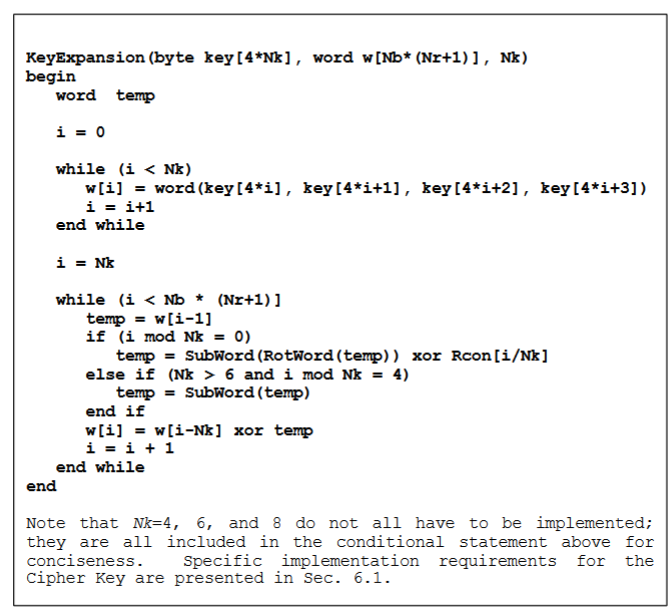
\includegraphics[width = 0.60\textwidth]{image8.png}
  \caption{Pseudoimplemetazione codice cifratura}
\end{figure}
\newpage

Viene allocato uno \textbf{scratchpad} di 2097152 bytes.\cite{crypto_note_standard_cryptonight}
Dall'output di Keccak vengono estratti i byte \texttt{64...191} e divisi
in 8 blocchi di 16 byte ciascuno. Ogni blocco viene cifrato utilizzando
il seguente codice:

\begin{algorithm}
  \caption{AES Rounds}
  \begin{algorithmic}[1]
  \For{$i = 0$ \textbf{to} $9$}
      \State block = \texttt{aes\_round}(block, round\_keys[$i$])
  \EndFor
  \end{algorithmic}
  \end{algorithm}


\subsubsection{Funzione cifratura AES}\label{funzione-cifratura-aes}

La funzione \texttt{aes\_round} esegue un round di cifratura AES, che
consiste nell'eseguire i passaggi seguenti sul blocco:

\begin{itemize}
\item
  SubBytes: ogni byte del blocco viene sostituito con un valore criptato
  utilizzando una tabella di sostituzione \emph{S-Box}.
\item
  ShiftRows: le righe del blocco vengono spostate di una posizione.
\item
  MixColumns: le colonne del blocco vengono mescolate utilizzando una
  matrice 4x4 nota come MDS, progettata per essere difficile
  da invertire.
\item
  Infine, il risultato è XORato con la chiave specifica per quel round.
  A differenza della classica funzione AES per cifrare, il primo e
  l'ultimo round quando si usano le \emph{round-keys} non sono speciali.
\end{itemize}

I blocchi che ne risultano vengono riportati nei primi 128 byte dello
scratchpad. Questi ultimi vengono cifrati nuovamente nello stesso modo,
e il risultato viene scritto nei successivi 128 byte. Questa operazione
viene effettuata 10 volte, per riempire tutto lo scratchpad di dati
pseudo-randomici. I byte \texttt{64..191}, che chiameremo
\emph{payload}, sono cifrati in questo modo 10 volte. Questo diagramma
mostra le operazioni effettuate in questa prima parte:

\begin{verbatim}
                               +-----+
                               |Input|
                               +-----+
                                  |
                                  V
                             +--------+
                             | Keccak |
                             +--------+
                                  |
                                  V
   +-------------------------------------------------------------+
   |                         Final state                         |
   +-------------+--------------+---------------+----------------+
   | Bytes 0..31 | Bytes 32..63 | Bytes 64..191 | Bytes 192..199 |
   +-------------+--------------+---------------+----------------+
          |                             |
          V                             |
   +-------------+                      V
   | Round key 0 |------------+---+->+-----+
   +-------------+            |   |  |     |
   |      .      |            |   |  |     |
   |      .      |            |   |  | AES |
   |      .      |            |   |  |     |
   +-------------+            |   |  |     |
   | Round key 9 |----------+-|-+-|->+-----+                 +---+
   +-------------+          | | | |     |                    |   |
                            | | | |     +------------------->|   |
                            | | | |     |                    |   |
                            | | | |     V                    |   |
                            | | | +->+-----+                 |   |
                            | | |    |     |                 | S |
                            | | |    |     |                 |   |
                            | | |    | AES |                 | c |
                            | | |    |     |                 |   |
                            | | |    |     |                 | r |
                            | | +--->+-----+                 |   |
                            | |         |                    | a |
                            | |         +------------------->|   |
                            | |         .                    | t |
                            | |         .                    |   |
                            | |         .                    | c |
                            | |         +------------------->|   |
                            | |         |                    | h |
                            | |         V                    |   |
                            | +----->+-----+                 | p |
                            |        |     |                 |   |
                            |        |     |                 | a |
                            |        | AES |                 |   |
                            |        |     |                 | d |
                            |        |     |                 |   |
                            +------->+-----+                 |   |
                                        |                    |   |
                                        +------------------->|   |
                                                             |   |
                                                             +---+
\end{verbatim}

Successivamente farò un immagine su questa cosa, ricordatemelo.

\subsection{Seconda parte: Loop
memory-hard}\label{seconda-parte-loop-memory-hard}

La seconda parte si compone di un algoritmo che mantiene lo stato
composto da 52488 iterazioni. Si utilizzano operazioni
CPU-friendly, come la cifratura AES, XOR, moltiplicazioni e addizioni di
8 byte, per avere come unico

Prima di eseguire il loop utilizzato per rendere questa funzione di hash
\emph{memory-hard}, viene eseguito lo XOR sui byte \texttt{0..31} e i
byte \texttt{32..63} dell'output dell'hashing Keccak. I 32 byte
risultanti vengono utilizzati per inizializzare due variabili da 16 byte
ciascuna, \texttt{a} e \texttt{b}. Queste variabili vengono utilizzate
nel loop principale, composte da quattro passaggi:

\begin{enumerate}
\def\labelenumi{\arabic{enumi}.}
\item
  Il codice calcola l'indirizzo di memoria della variabile \texttt{a} e
  lo scrive sullo scratchpad. Per convertire un valore di 16 byte in un
  indirizzo nello scratchpad, bisogna interpretarlo come un intero
  rappresentato in little-endian, con gli ultimi 21 bit che
  rappresentano l'indice all'interno dei byte; gli ultimi 4 bit vengono
  comunque cancellati per ottenere l'allinamento a 16 byte, dato che i
  dati vengono letti e scritti sullo scratchpad in blocchi da 16 byte.
\item
  Successivamente, viene applicatata la funzione per cifrare il blocco
  \texttt{aes\_round} sull'indirizzo letto dallo scratchpad, con il
  valore di \texttt{a} usato come chiave.
\item
  Il risultato di questa operazione passa da uno XOR e il valore della
  variabile \texttt{b}, oltre ad essere scritto sullo scratchpad, sempre
  come indirizzo di memoria.
\item
  L'indirizzo ricavato viene letto dallo scratchpad e viene effettuata
  l'operazione di moltiplicazione chiamata \texttt{8byte\_mul}. Questa
  funzione, usa i primi 8 byte di ogni argomento, interpretati da essa
  come \texttt{uint\_64}, con rappresentazione little-endian. Il
  risultato di questa operazione viene convertito in 16 byte,
  concludendo l'operazione di moltiplicazione scambiando le due metà del
  risultato (8 byte ciascuna)
\item
  Il valore di \texttt{a} viene aggiunto, componente per componente in
  modulo 2\^{}64, al risultato della moltiplicazione con le due metà già
  scambiate attraverso la funzione \texttt{8byte\_add} che utilizza i
  primi 64 bit come intero senza segno, con il risultato che viene
  portato in 16 byte e scritto nello scratchpad.
\item
  Infine, viene letto l'indirizzo del risultato della cifratura
  dell'indirizzo della variabile di \texttt{a}, utilizzando come chiave
  \texttt{a} (il risultato del secondo passaggio) e viene effettuata un
  operazione di XOR con il risultato della addizione precedente.
\item
  Il risultato dell'operazione 6 viene utilizzato come nuovo valore
  della variabile \texttt{a}, mentre il risultato del passaggio 2 viene
  utilizzato come nuova variabile \texttt{b}.
\end{enumerate}

Il diagramma presente illustra le operazioni eseguite nel loop
\emph{memory-hard}:

\begin{verbatim}
   +-------------------------------------------------------------+
   |                         Final state                         |
   +-------------+--------------+---------------+----------------+
   | Bytes 0..31 | Bytes 32..63 | Bytes 64..191 | Bytes 192..199 |
   +-------------+--------------+---------------+----------------+
          |             |
          |   +-----+   |
          +-->| XOR |<--+
              +-----+
               |   |
          +----+   +----+
          |             |
          V             V
        +---+         +---+
        | a |         | b |
        +---+         +---+
          |             |
   --------------------- REPEAT 524288 TIMES ---------------------
          |             |                            address +---+
          +-------------|----------------------------------->|   |
          |   +-----+   |                               read |   |
          +-->| AES |<--|------------------------------------|   |
          |   +-----+   V                                    |   |
          |      |   +-----+                                 | S |
          |      +-->| XOR |                                 |   |
          |      |   +-----+                           write | c |
          |      |      |    +------------------------------>|   |
          |      |      +----+                       address | r |
          |      +------------------------------------------>|   |
          |      |  +-----------+                       read | a |
          |      +->| 8byte_mul |<--+------------------------|   |
          |      |  +-----------+   |                        | t |
          |      |        |         |                        |   |
          |      |        V         |                        | c |
          |      |  +-----------+   |                        |   |
          +------|->| 8byte_add |   |                        | h |
                 |  +-----------+   |                        |   |
                 |        |         |                  write | p |
                 |        +---------|----------------------->|   |
                 |        |         |                        | a |
                 |        V         |                        |   |
                 |     +-----+      |                        | d |
                 |     | XOR |<-----+                        |   |
                 |     +-----+                               |   |
                 +------+ |                                  |   |
          +-------------|-+                                  |   |
          |             |                                    +---+
   -------------------------- END REPEAT -------------------------
\end{verbatim}

\subsection{Terza parte: Calcolo del
risultato}\label{terza-parte-calcolo-del-risultato}

Dopo aver effettuato le operazioni memory-hard, i byte \texttt{32..63}
dati dall'hashing effettuato con Keccak vengono espansi in 10
\emph{round-keys} come nella prima parte.

I byte \texttt{64..191} dello stesso hashing vengono presi e viene
effettuato uno XOR con i primi 128 byte dello scratchpad. Il risultato
di questa operazione viene criptato con la funzione \texttt{aes\_round}
come nella prima parte, ma con le chiavi ricavate dall'espansione dei
byte \texttt{32..63}.\\
Il risultato di questa cifratura viene passato da uno XOR con i 128
bytes successivi dello scratchpad, cifrati nuovamente con la stessa
funzione, fino ad arrivare agli ultimi 128 byte dello scratchpad. Dopo
aver cifrato gli ultimi 128 byte viene effettuato lo XOR con gli ultimi
128 byte dello scratchpad.

I byte \texttt{64..191} del **Keccak state* vengono sostituiti con Il
risultato dell'operazione effettuata in precedenza. Tutti i 200 byte
dello stato di Keccak vengono passati da una permutazione, chiamata
\emph{Keccak-f}, con parametro \texttt{b\ =\ 1600}, l'implementazione
più sicura. Questa operazione viene effettuate per mescolare i bit dello
stato Keccak, in modo da rendere difficile la criptoanalisi del flusso
di dati.

Infine, i due bit più a destra vengono utilizzati per selezionare una
funzione di hash:

\begin{itemize}
  \item 
  0: BLAKE-256\cite{aumasson2008sha}
  \item
  1: Groest1-256\cite{groestl}
  \item 
  2: JH-256\cite{jh}
  \item 
  3: Skein-256\cite{skein}
\end{itemize}

L'output di questa funzione di hash viene applicato al Keccak state, e
l'hash risultante è l'output di CryptoNight. Il diagramma sottostante
rappresenta il calcolo del risultato:
\begin{verbatim}
 +-------------------------------------------------------------+
   |                         Final state                         |
   +-------------+--------------+---------------+----------------+
   | Bytes 0..31 | Bytes 32..63 | Bytes 64..191 | Bytes 192..199 |
   +-------------+--------------+---------------+----------------+
         |                |             |                |
         |       +--------+             |                |
         |       V        |             |                |
         |+-------------+ |             |                |
         || Round key 0 |-|---+---+     |                |
         |+-------------+ |   |   |     |                |
         ||      .      | |   |   |     |                |
         ||      .      | |   |   |     |                |
         ||      .      | |   |   |     |                |
         |+-------------+ |   |   |     |                |
   +---+ || Round key 9 |-|-+-|-+ |     V                |
   |   | |+-------------+ | | | | |  +-----+             |
   |   |-|----------------|-|-|-|-|->| XOR |             |
   |   | |                | | | | |  +-----+             |
   | S | |                | | | | |     |                |
   |   | |                | | | | |     V                |
   | c | |                | | | | +->+-----+             |
   |   | |                | | | |    |     |             |
   | r | |                | | | |    |     |             |
   |   | |                | | | |    | AES |             |
   | a | |                | | | |    |     |             |
   |   | |                | | | |    |     |             |
   | t | |                | | | +--->+-----+             |
   |   | |                | | |         |                |
   | c | |                | | |         V                |
   |   | |                | | |      +-----+             |
   | h |-|----------------|-|-|----->| XOR |             |
   |   | |                | | |      +-----+             |
   | p | |                | | |         |                |
   |   | |                | | |         .                |
   | a | |                | | |         .                |
   |   | |                | | |         .                |
   | d | |                | | |         |                |
   |   | |                | | |         V                |
   |   | |                | | |      +-----+             |
   |   |-|----------------|-|-|----->| XOR |             |
   |   | |                | | |      +-----+             |
   +---+ |                | | |         |                |
         |                | | |         V                |
         |                | | +----->+-----+             |
         |                | |        |     |             |
         |                | |        |     |             |
         |                | |        | AES |             |
         |                | |        |     |             |
         |                | |        |     |             |
         |                | +------->+-----+             |
         |                |             |                |
         V                V             V                V
   +-------------+--------------+---------------+----------------+
   | Bytes 0..31 | Bytes 32..63 | Bytes 64..191 | Bytes 192..199 |
   +-------------+--------------+---------------+----------------+
   |                       Modified state                        |
   +-------------------------------------------------------------+
                                  |
                                  V
                            +----------+
                            | Keccak-f |
                            +----------+
                             |    |
                 +-----------+    |
                 |                |
                 V                V
          +-------------+  +-------------+
          | Select hash |->| Chosen hash |
          +-------------+  +-------------+
                                  |
                                  V
                          +--------------+
                          | Final result |
                          +--------------+
\end{verbatim}